\documentclass[a4paper,14pt]{extarticle} \usepackage[utf8]{inputenc}
\usepackage[T1]{fontenc}
\usepackage[margin=2.5cm]{geometry}

% Fonte Caladea se existir, senão lmodern
\IfFileExists{caladea.sty}{
  \usepackage{caladea}
}{
  \usepackage{lmodern} }
\usepackage{ragged2e}
\usepackage{graphicx}
\usepackage[portuguese]{babel}
\usepackage{wrapfig}
\usepackage{hyperref}
\usepackage{fancyhdr}
\usepackage{xcolor}
\usepackage{rotating}
\usepackage{titlesec}
\usepackage{epigraph}
\usepackage{dirtytalk}
\usepackage{indentfirst} % Indenta o primeiro parágrafo após seções

% Ajuste do recuo de parágrafo
\setlength{\parindent}{1.5em}

% Centralizar títulos
\titleformat{\section}
  {\normalfont\centering\bfseries\Large}{\thesection}{1em}{}

\titleformat{\subsection}
  {\normalfont\centering\bfseries\large}{\thesubsection}{1em}{}

\titleformat{\subsubsection}
  {\normalfont\centering\bfseries}{\thesubsubsection}{1em}{}

% -------------- Símbolos de Versículo e Resposta --------------
% Definição do símbolo (a “barrinha” inclinada)
\makeatletter
\newcommand{\vers@resp@sym}{%
  \raisebox{0.2ex}{\rotatebox[origin=c]{-20}{$\m@th\rceil$}}%
}
% macro interna que sobrepõe a barrinha e a letra V ou R
\newcommand{\vers@resp}[2]{%
  {\ooalign{%
     \hidewidth\kern#1\vers@resp@sym\hidewidth\cr
     #2\cr
  }}%
}
% comandos públicos \versicle e \response
\DeclareRobustCommand{\versicle}{\vers@resp{-0.1em}{V}}
\DeclareRobustCommand{\response}{\vers@resp{0pt}{R}}
\makeatother
% ^------------- Símbolos de Versículo e Resposta -------------^

% Rodapé com imagem e página
\pagestyle{fancy}
% ---- Cabeçalho ------------
\fancyhf[C]{}
% ----- Rodapé --------------
\fancyfoot[LO,LE]{%
  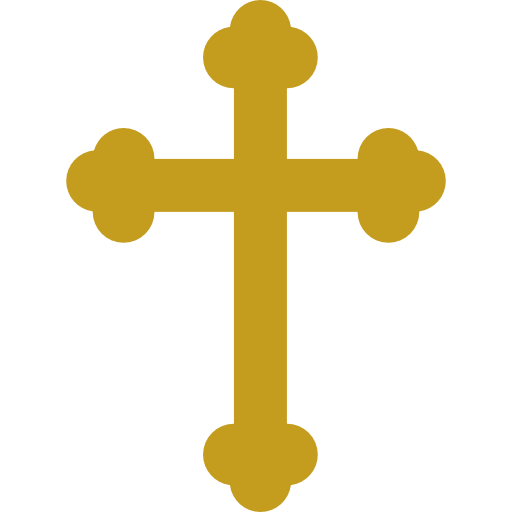
\includegraphics[scale=0.2]{assets/cross.png}\quad
  \textit{Novena a \textbf{São Carlo Acutis}}
}
\fancyfoot[RO,RE]{\thepage}

\begin{document}


\begin{center}
  {\huge Novena a São Carlo Acutis}
\end{center}

\say{
Carlo era um garoto absolutamente normal. Fazia as coisas que todas as crianças de hoje fazem: usava o computador, brincava com os amigos, levava uma vida semelhante à dos seus amigos.
A única grande diferença é que havia colocado no centro de seu dia o encontro com Jesus Eucarístico com a Missa e da Adoração que fazia sempre antes ou depois da celebração.

A Eucaristia diária tornou-se uma necessidade real para ele. Sua frase famosa é: "\textbf{A Eucaristia é a minha autoestrada para o céu}". Dizia que todos nós somos chamados a sermos discípulos amados como João o Apóstolo, o grande cantor da Eucaristia.
}

\par\noindent\rule{\textwidth}{0.4pt}

\tableofcontents
\thispagestyle{empty}

% --- Vida / Origem da Novena ---
\newpage

\section{História do Santo}

Carlo Acutis é o primeiro santo da geração millennial. Ele nasceu em Londres (Reino Unido) em 3 de maio de 1991. Na época, seus pais, ambos originários da Itália, moravam em Londres, onde seu pai trabalhava. Carlo foi batizado duas semanas após seu nascimento.

No outono daquele ano, a família retornou a Milão, onde Carlo frequentou a escola primária no Instituto Tommaseo, administrado pelas Irmãs de Santa Marcelina (Marcelinas). Ele foi autorizado a receber sua Primeira Comunhão aos sete anos de idade no Mosteiro das Eremitas Ambrosianas em Bernaga di Perego (Lecco).

Ao longo de sua vida, Carlo demonstrou profunda devoção à Eucaristia. Participava da Missa todos os dias e fazia uma "comunhão espiritual" nos dias em que estava ocupado com os estudos. Frequentemente realizava pequenos sacrifícios em reparação pela falta de amor demonstrada a Jesus na Eucaristia e contava histórias sobre isso aos seus amigos. Suas palavras, "A Eucaristia é minha auto-estrada para o céu", tornaram-se famosas.

Após o ensino fundamental, matriculou-se no clássico Instituto Leone XIII, em Milão, fundado pela Companhia de Jesus. Além de suas atividades escolares, foi catequista em sua paróquia, Santa Maria Segreta, em Milão, onde aprendeu a projetar e criar páginas web enquanto trabalhava no site da paróquia com um aluno de engenharia da computação. Desenvolveu tamanha paixão por esse tipo de trabalho que, no verão de 2006, projetou um site para um projeto de promoção do voluntariado em sua escola e trabalhou na página da Pontifícia Academia \textit{Cultorum Martyrum}, da qual sua mãe participava. Ele também usou o computador para criar um layout para a oração do Rosário, mas o mais impressionate de seus trabalhos certamente é a exposição internacional sobre os \href{https://www.miracolieucaristici.org/pr/Liste/list.html}{\color{blue}\underline{milagres eucarísticos}} ao redor do mundo, em que ele, junto de seus pais, por vezes viajou a diversos cantos da Europa para estudar os milagres reconhcidos pela Igreja, formando uma admirável coleção de documentos ao longo de alguns anos que resumem a história de dezenas de milagres.

Carlo era um adolescente alegre e extrovertido, de bom coração. Não escondia sua fé e seu amor por Jesus. Estava sempre disposto a ajudar um colega necessitado e era amigo dos pobres de sua vizinhança, dando-lhes parte de sua mesada quando pediam ajuda. Ele costumava dizer: "Estar sempre perto de Jesus, esse é o meu projeto de vida". Enquanto passava parte das férias de verão em Assis (Perúgia), adotou a espiritualidade franciscana de alegria, contemplação e respeito pela criação, busca pela paz e proximidade com os mais necessitados.

Em outubro de 2006, foi diagnosticado com uma forma agressiva de leucemia. Em poucos dias, sua saúde piorou. Ele ofereceu seu sofrimento ao Santo Padre, pelo bem da Igreja e pela esperança de ir para o céu. Após ser internado no Hospital San Gerardo, em Monza, recebeu o Sacramento da Unção dos Enfermos. Em 12 de outubro de 2006, aos 15 anos e 5 meses, Carlo faleceu.

Seu corpo foi sepultado inicialmente no túmulo da família em Ternengo (Biella) e, posteriormente, transferido para o cemitério de Assis. Há alguns anos, ele é conservado no Santuário do Despojamento, na mesma cidade de São Francisco, onde é exposto à veneração de um grande número de fiéis provenientes de todo o mundo.

Apenas cinco anos após a morte de Carlo, foi fundada em Milão a Associação "Amigos de Carlo Acutis", com o objetivo de promover sua causa de beatificação e canonização. A investigação diocesana foi realizada em Milão entre 2013 e 2016 e, em 5 de julho de 2018, o Papa Francisco autorizou a então Congregação para as Causas dos Santos a promulgar o decreto declarando que Carlo havia praticado as virtudes cristãs em grau heroico.

Sucessivamente, o mesmo Papa reconheceu o primeiro milagre atribuído à intercessão de Carlo, ocorrido  na Arquidiocese de Campo Grande (Brasil), em 2013. Isso possibilitou a celebração de sua beatificação em 10 de outubro de 2020, na Basílica Superior de São Francisco, em Assis.

Por fim, o Papa Francisco, ao aprovar um segundo milagre realizado por Deus por intercessão do Beato Carlo Acutis, ocorrido em Florença em 2022, abriu caminho para sua canonização.


% --- Orações Diárias ---
\newpage

\section{Novena São Carlo Acutis}

\subsection{Oração Inicial} \label{oracao-inicial}

Santíssima Trindade, Pai, Filho e Espírito Santo, eu vos agradeço por todos os favores e todas as graças com que enriquecestes a alma de São Carlo Acutis durante os 15 anos que passou nesta Terra e, pelos méritos deste tão querido Anjo da Juventude, vos suplico que me concedais a graça que ardentemente vos peço: (faz-se o pedido da graça que se deseja).

\subsection{Meditação do Primeiro Dia}

Começar com a \textbf{\nameref{oracao-inicial}.}

“Não eu, mas Deus”

São Carlo Acutis, que fizeste de tua vida uma contínua renúncia e aniquilamento, dá-me a graça de buscar as coisas do Céu e desprezar as que passam. Amém.

Terminar com a \textbf{\nameref{oracao-final}.}

\subsection{Meditação do Segundo Dia}

Começar com a \textbf{\nameref{oracao-inicial}.}

“Estar sempre junto com Jesus: este é o meu plano de vida”

São Carlo Acutis, que viveste imerso no Coração de Jesus, dá-me a graça de realizar, em tudo, este teu plano de amor. Amém.

Terminar com a \textbf{\nameref{oracao-final}.}

\subsection{Meditação do Terceiro Dia}

Começar com a \textbf{\nameref{oracao-inicial}.}

“Peça ao seu Anjo da Guarda para ajudá-lo continuamente, de modo que ele se torne seu melhor amigo.”

São Carlo Acutis, que buscaste, já neste mundo, a companhia dos santos anjos, dá-me a graça de viver na retidão que o meu santo anjo deseja. Amém.

Terminar com a \textbf{\nameref{oracao-final}.}

\subsection{Meditação do Quarto Dia}

Começar com a \textbf{\nameref{oracao-inicial}.}

“Nossa alma é como um balão… Se por acaso existe um pecado mortal, a alma cai sobre a Terra e a confissão será como fogo… É preciso confessar-se frequentemente.”

São Carlo Acutis, que tão bem viveste o sacramento da reconciliação, dá-me a graça de buscá-lo sempre com uma contrição profunda. Amém.

Terminar com a \textbf{\nameref{oracao-final}.}

\subsection{Meditação do Quinto Dia}

Começar com a \textbf{\nameref{oracao-inicial}.}

“A tristeza é a visão voltada para si; a felicidade é seu olhar para Deus.”

São Carlo Acutis, que jamais desviaste o teu olhar de Jesus, teu grande amor, dá-me a graça de viver já neste mundo esta verdadeira felicidade. Amém.

Terminar com a \textbf{\nameref{oracao-final}.}

\subsection{Meditação do Sexto Dia}

Começar com a \textbf{\nameref{oracao-inicial}.}

“A única coisa que nós temos que pedir a Deus na oração é a vontade de ser santos”

São Carlo Acutis, que soubeste sempre pedir a Deus o essencial, dá-me a graça de um profundo desejo do Céu. Amém.

Terminar com a \textbf{\nameref{oracao-final}.}

\subsection{Meditação do Sétimo Dia}

Começar com a \textbf{\nameref{oracao-inicial}.}

“A Virgem Maria é a única mulher da minha vida”

São Carlo Acutis, que amaste a Virgem Maria mais que tudo, dá-me a graça de corresponder ao amor desta tão terna e boa mãe. Amém.

Terminar com a \textbf{\nameref{oracao-final}.}

\subsection{Meditação do Oitavo Dia}

Começar com a \textbf{\nameref{oracao-inicial}.}

“A Eucaristia é a minha estrada para o Céu”

São Carlo Acutis, que buscavas sempre teu Jesus escondido no sacrário, dá-me a graça de um profundo ardor eucarístico. Amém.

Terminar com a \textbf{\nameref{oracao-final}.}

\subsection{Meditação do Nono Dia}

Começar com a \textbf{\nameref{oracao-inicial}.}

“Eu estou feliz de morrer, porque vivi a minha vida sem perder nenhum minuto em coisas que não agradam a Deus”

São Carlo Acutis, dá-me a graça das graças, que é a perseverança final e uma morte santa. Amém.

Terminar com a \textbf{\nameref{oracao-final}.}


\subsection{Oração Final} \label{oracao-final}
\begin{center}
Rezam-se \textbf{5 Pai-Nossos, 5 Ave-Marias, 5 Glória Ao Pais} em honra aos 15 anos de de vida de São Carlo Acutis. 
\end{center}

\textbf{Oremos:} Deus Pai de Misericórdia, que elevastes à glória dos altares este vosso servo Carlo Acutis, a fim de que, por ele, vós fôsseis mais glorificado, concedei-nos, pelos méritos dele — que em tudo viveu a vossa vontade —, a graça que ardentemente desejo. Amém.

\[
  \textbf{São Carlo Acutis, rogai por nós!}
\]

\vfill

\begin{center}
\subsection*{Fontes:}
Adaptado de: \underline{\href{https://bibliotecacatolica.com.br/blog/carlo-acutis/novena-carlo-acutis/}{Minha Biblioteca Católica}} e \underline{\href{https://www.vaticannews.va/pt/papa/news/2025-09/papa-leao-xiv-missa-canonizacao-biografia-acutis.html}{Vatican News}}.
\end{center}


\end{document}
